\documentclass[11pt,a4paper]{article}

% --- Mathematics (must precede unicode-math) ---
\usepackage{amsmath}
\usepackage{mathtools}

% --- Fonts (lualatex) ---
\usepackage{fontspec}
\usepackage{unicode-math}
\setmathfont{KpMath-Regular.otf}
\setmathfont{KpMath-Bold.otf}[version=bold]

\usepackage{microtype}
\usepackage[dvipsnames]{xcolor}
\usepackage[margin=25mm, top=30mm, bottom=30mm]{geometry}

\usepackage{fancyhdr}
\pagestyle{fancy}
\fancyhf{}
\fancyhead[L]{\small\itshape The Single-Site T-Matrix of a Legendre Cell}
\fancyhead[R]{\small\itshape Nestor (2026)}
\fancyfoot[C]{\thepage}
\renewcommand{\headrulewidth}{0.4pt}
\renewcommand{\footrulewidth}{0pt}

\setcounter{secnumdepth}{3}
\usepackage{booktabs}
\usepackage{array}
\usepackage{graphicx}
\usepackage{placeins}
\usepackage[numbers,sort&compress]{natbib}
\usepackage[font=small, labelfont=bf, labelsep=period]{caption}
\usepackage{setspace}
\setstretch{1.15}
\setlength{\parskip}{0.4em}
\usepackage[colorlinks=true, linkcolor=blue!60!black,
            citecolor=blue!60!black, urlcolor=blue!60!black]{hyperref}

% --- Macros ---
\newcommand{\bK}{\mathbf{K}}
\newcommand{\bG}{\mathbf{G}}
\newcommand{\bE}{\mathbf{E}}
\newcommand{\bF}{\mathbf{F}}
\newcommand{\bM}{\mathbf{M}}
\newcommand{\bN}{\mathbf{N}}
\newcommand{\bT}{\mathbf{T}}
\newcommand{\bI}{\mathbf{I}}
\newcommand{\bx}{\mathbf{x}}
\newcommand{\by}{\mathbf{y}}
\newcommand{\bs}{\mathbf{s}}
\newcommand{\bD}{\boldsymbol{\Delta}}
\newcommand{\biota}{\boldsymbol{\iota}}
\newcommand{\bxi}{\boldsymbol{\xi}}
% the differential of every integral and derivative is upright: \dd z, \dd^3x, \frac{\dd}{\dd z}
\newcommand{\dd}{\mathrm{d}}

\title{\bfseries The Single-Site T-Matrix of a Legendre Cell in Closed Form\\[4pt]
\large Elastic Waves, Every Power of the Frequency on Six Constants}
\author{T. M. Nestor\\[2pt]\small Independent researcher, Australia}
\date{Draft, 7 October 2026}

\begin{document}
\maketitle

\begin{abstract}
\noindent
A volume-integral method for elastic waves divides a heterogeneous medium into cells, each with a
single-site $T$-matrix that maps the field incident on it to the sources it radiates. The governing
equation is written in displacement; how the strain inside a cell is represented is a modelling
decision, and the original approximation takes it as uniform. We take the cell whose displacement and
strain are independent Legendre expansions over the cube, tested against the same polynomials (a Galerkin
cell), because of the representations in use it gives the most accurate coupling between cells: its
interactions are exact double integrals over both cells, where an expansion about the cell's centre treats
the receiving cell as a point. For the linear Legendre cell with a uniform contrast we give the single-site
$T$-matrix in closed form at every power of the wavenumber. Its self-interaction is a power series,
$\mathbf K=\sum_n(k_Sh)^n\mathbf K_n$ with $h$ the half-width, whose coefficients $\mathbf K_n$ are moments of
powers of the distance over the cell and depend on neither the frequency, the cell size nor the medium.
Every coefficient is exact: an even power of $k_Sh$ is a combination with rational coefficients of six constants,
$1$, $\pi$, $\sqrt2$, $\sqrt3$, $\ln(1+\sqrt2)$ and $\ln(2+\sqrt3)$, the last two the logarithms of the
fundamental units of $\mathbb Q(\sqrt2)$ and $\mathbb Q(\sqrt3)$, and an odd power,
which carries the radiation, is rational. The first of these is the radiation damping of a point force,
recovered exactly. On the irreducible representations of the cube group the $36$ unknowns of the cell
separate into blocks of at most four, and the $T$-matrix becomes a handful of closed-form matrices per
power of $k_Sh$. Through $(k_Sh)^6$ the closed form reproduces the $T$-matrix computed by quadrature to
$3.5\times10^{-9}$ at $k_Sh=0.2$, falling as $(k_Sh)^7$ as the next term predicts, and each of its $223$
moments to $1.7\times10^{-15}$. Because the coefficients depend on neither the frequency, the cell size nor
the medium, a frequency sweep integrates nothing at any frequency: the $T$-matrix costs $0.3$\,ms per frequency
against $2$\,s by quadrature, after a one-off derivation of $30$\,s.
\end{abstract}

% =====================================================================================================
% DRAFT STATUS (7 October 2026). Written from the derivation in scripts/derive_legendre_cell_dynamic.py,
% whose checks all pass, and from the single-cell section of the coupling paper (Paper 2, sec:site and
% app:blocks), which this paper takes over. Scope as planned in docs/2026-10-07-three-paper-split-plan.md
% (decision D7). To come: the graded contrast in the cell; the quadratic field; the comparison with the
% collocated (hierarchy) single site, condensed from the earlier Paper 1; declarations as in Papers 1-2.
% =====================================================================================================

\section{Introduction}\label{sec:intro}

A volume-integral method for elastic scattering replaces a heterogeneous medium by cells, here cubes, and
couples them through the Green's tensor of the background. Each cell is characterised by its single-site
$T$-matrix: the map from the field incident on it to the sources it radiates when it is alone. The coupled
system is then the multiple-scattering problem of the cells
\citep{Foldy1945,Lax1951,Waterman1976,MishchenkoTravisLacis2002}, and everything that a cell contributes to
the solution, beyond its coupling to the others, is in its $T$-matrix.

How the field inside a cell is represented decides what that $T$-matrix is. The governing equation is
written in displacement, and the strain enters it only through the stiffness contrast; how the strain is
represented within a cell is therefore a modelling decision. The original approximation, of the
equivalent-inclusion method \citep{Eshelby1957,Mura1987} and of the coupled-dipole method for elastic
waves \citep{Nestor1996}, takes it as uniform. That approximation can be relaxed in two ways. In the
first, the displacement is expanded about the cell's centre and the strain derived from it; the equation
and its derivatives are imposed at the centre, which is natural for a single scatterer, whose $T$-matrix is
then a property of the body alone \citep{NestorContinuum2026}. In the second, the strain is an unknown in
its own right, with its own polynomial expansion over the cell, and the equation is tested against the
cell's polynomials (a Galerkin cell). Which of the two a tiling of cells needs is measured on a layer, which
has an exact solution (Table~\ref{tab:strainlayer}): with polynomials of degree $p$, an independent strain
converges at order $2p+2$, while a strain derived from each cell's displacement converges at order $2$, $2$
and $4$ for $p=1$, $2$ and $3$.

This paper takes the second, because it gives the more accurate representation of the coupling between
cells. Its interactions are exact double integrals over both cells, which are evaluated to round-off even
for cells that touch \citep{NestorCoupling2026}; an expansion about the centre treats the receiving cell as
a point. On a cube cut into $n^3$ cells, where the field follows the corners, the first-moment Legendre
cell of $36$ unknowns is seven to twelve times more accurate than the third-gradient expansion about the
centre with $60$; on a smoothly graded sphere both converge at fourth order, and the Legendre cell is the
more accurate for a given number of unknowns \citep{NestorContinuum2026}. And a Galerkin cell holds the
projection of the field and of the medium, which is what makes its error a projection error, known before
the solve \citep{NestorError2026}.

The single-site $T$-matrix of the linear Legendre cell was given in \citet{NestorCoupling2026} in its
static limit, entry by entry on five constants. Here it is given at every power of the frequency. The
central result is that the self-interaction of the cell, the only part of its $T$-matrix that is an
integral, is
\begin{equation}\label{eq:centralresult}
  \bK=\sum_{n\ge0}(k_Sh)^n\,\bK_n ,\qquad \bK_n\ \text{exact for every }n,
\end{equation}
a power series in $k_Sh$ whose coefficients are universal moments of powers of the distance over the cell
\citep{NestorCoupling2026}, independent of the frequency, the cell size and the medium. We evaluate every one
of them exactly (\S\ref{sec:moments}), and find that each even power of $k_Sh$ is a combination with
rational coefficients of the same six constants and that each odd power, which carries the radiation, is
rational (\S\ref{sec:constants}). Computed once and stored, the $\bK_n$ give the $T$-matrix at any frequency
without an integral (\S\ref{sec:discussion}). The cube group reduces the $36$ unknowns to blocks of at most four
(\S\ref{sec:group}, Figure~\ref{fig:blocks}), on which the $T$-matrix is a few closed-form matrices per
power. Section
\ref{sec:checks} gives the checks, each against an evaluation that shares no step with the closed form.

\section{The cell and its single-site matrix}\label{sec:cell}

\paragraph{The governing equation.} With time dependence $\mathrm e^{-\mathrm i\omega t}$, split the
density and the stiffness into the background and the contrast, $\rho=\rho_0+\Delta\rho$ and
$c=c^0+\delta c$, $\delta c_{bcde}=\Delta\lambda\,\delta_{bc}\delta_{de}
+\Delta\mu(\delta_{bd}\delta_{ce}+\delta_{be}\delta_{cd})$. The contrast acts on the background as a body
force, $\omega^2\Delta\rho\,u_b+\partial_cm_{bc}$ with $m_{bc}=\delta c_{bcde}\varepsilon_{de}$, and with
$\bG$ the background's Green's tensor the displacement is
\begin{equation}\label{eq:ls}
  u_a(\bx)=u^0_a(\bx)+\int G_{ab}(\bx-\by)\,\omega^2\Delta\rho\,u_b(\by)\,\dd^3y
  +\int\frac{\partial G_{ab}}{\partial x_c}(\bx-\by)\,m_{bc}(\by)\,\dd^3y ,
\end{equation}
the moment radiating through the receiver derivative of $\bG$ \citep{NestorContinuum2026}. The strain
enters only through $m$. Differentiating Eq.~\eqref{eq:ls} gives the strain at $\bx$, and the pair
$\psi=(u,\varepsilon)$, nine components with the strain in engineering Voigt form, satisfies one
Lippmann--Schwinger equation with a $9\times9$ kernel and the contrast operator
$\bD=\operatorname{blockdiag}(\omega^2\Delta\rho\,\bI_3,\Delta\mathcal C)$, $\Delta\mathcal C$ the Voigt
form of $\delta c$ \citep{NestorContinuum2026}.

\paragraph{The strain model.} Table~\ref{tab:strainmodel} sets out the three representations of the strain
that this series meets. They differ in the unknowns, and the test of the equation follows from the
unknowns: derivatives at a point are fixed by imposing the equation and its derivatives there, moments over
a cell by testing against the cell's own polynomials. This paper is about the third.

\begin{table}[htbp]
\centering
\caption{How the strain is represented within a cell, and the test that follows. The words
\emph{collocation} and \emph{Galerkin} describe only the test.}\label{tab:strainmodel}
\small
\begin{tabular}{@{}p{3.1cm}p{4.3cm}p{3.9cm}p{3.2cm}@{}}
\toprule
strain model & unknowns of a cell & strain and displacement & test \\
\midrule
uniform (the original approximation) & displacement and strain at the centre & strain uniform & at the
centre \\
derived & $\partial^Pu$ at the centre, $|P|\le\ell$ & strain the gradient of a Taylor displacement, degree
$\ell-1$ & the equation and its derivatives at the centre \\
independent (this paper) & Legendre moments of displacement and strain to degree $p$ & independent, both
degree $p$ & against the cell's polynomials (Galerkin) \\
\bottomrule
\end{tabular}
\end{table}

\begin{table}[htbp]
\centering
\caption{Derived against independent strain, on a layer of thickness $D$ with an exact solution (P wave at
normal incidence, $k_PD=0.6$, $\Delta(\lambda+2\mu)=4$\,GPa, $\Delta\rho=100$\,kg\,m$^{-3}$): relative error of
the reflected displacement with $16$ and $32$ cells, and the order between them. All three schemes use
Legendre polynomials of degree $p$ in each cell, tested against the same. \emph{Independent}: displacement
and strain each of degree $p$. \emph{Derived}: displacement of degree $p$, strain its derivative in each cell.
\emph{Derived, with faces}: the same, with the jumps of the displacement across the faces between cells added
to the stiffness source as plane deltas, which makes the derivative that of a distribution.}\label{tab:strainlayer}
\small
\begin{tabular}{@{}lccccccccc@{}}
\toprule
 & \multicolumn{3}{c}{independent} & \multicolumn{3}{c}{derived} & \multicolumn{3}{c}{derived, with faces} \\
\cmidrule(lr){2-4}\cmidrule(lr){5-7}\cmidrule(l){8-10}
$p$ & $n=16$ & $32$ & order & $16$ & $32$ & order & $16$ & $32$ & order \\
\midrule
$1$ & $2.6\times10^{-9}$ & $1.6\times10^{-10}$ & $4.00$ & $9.0\times10^{-5}$ & $2.2\times10^{-5}$ & $2.00$ &
$1.4\times10^{-4}$ & $3.6\times10^{-5}$ & $1.98$ \\
$2$ & $2.6\times10^{-14}$ & round-off & $6.00^{\,a}$ & $1.4\times10^{-5}$ & $3.5\times10^{-6}$ & $2.00$ &
$7.7\times10^{-7}$ & $9.5\times10^{-8}$ & $3.01$ \\
$3$ & round-off & round-off & $7.96^{\,b}$ & $8.2\times10^{-10}$ & $5.1\times10^{-11}$ & $4.00$ &
$1.4\times10^{-9}$ & $8.8\times10^{-11}$ & $3.98$ \\
\bottomrule
\end{tabular}

\smallskip
{\footnotesize $^a$ from $4$ to $8$ cells. $^b$ from $2$ to $4$ cells; finer grids are at round-off.}
\end{table}

The derived strain loses most of the order: at $16$ cells its errors are $3\times10^4$ times those of the
independent strain for $p=1$ and $5\times10^8$ times for $p=2$
(\path{scripts/measure_derived_vs_independent_strain.py}). Restoring the jumps of the cellwise displacement across the faces does not recover
it, so the loss is not the faces' alone; with the strain an unknown of its own, tested against the same
polynomials as the displacement, the scheme reaches the order $2p+2$ that a Galerkin scheme gives a
functional of its solution \citep{NestorContinuum2026}.

\paragraph{The linear Legendre cell.} A cube $[-h,h]^3$ with local coordinates $\bxi=(\bx-\bx_c)/h$ carries
$\psi(\bx)=\sum_b\psi_bL_b(\bxi)$ over the four functions $L_b\in\{1,\xi_0,\xi_1,\xi_2\}$, each $\psi_b$ a
nine-component vector: $36$ unknowns. With the contrast uniform in the cell the source density
$\bD\psi$ is a polynomial on the same four functions. Testing Eq.~\eqref{eq:ls} and its derivative against
each $L_a$ gives the single-site equation \citep{NestorCoupling2026}
\begin{equation}\label{eq:sitels}
  \bigl(\bM-\bK\bD\bigr)\psi=\langle L,\psi^0\rangle,\qquad \bM_{ab}=\langle L_a,L_b\rangle\,\bI_9,
\end{equation}
with $\bM=\operatorname{diag}(8h^3,\tfrac83h^3,\tfrac83h^3,\tfrac83h^3)\otimes\bI_9$ and $\bK$ the self block,
the kernel integrated against $L_a$ over the cell as receiver and $L_c$ over the cell as source. The
single-site matrix maps the Legendre coefficients of the incident field to the source moments
$\sigma_a=\langle L_a,\bD\psi\rangle$, the mean force and stress and their first moments,
\begin{equation}\label{eq:t36}
  \bT_{36}=\bM\bD\bigl(\bM-\bK\bD\bigr)^{-1}\bM=\bM\bD\bigl(\bI-\bN\bD\bigr)^{-1},\qquad\bN=\bM^{-1}\bK .
\end{equation}
Everything specific to the cube is in $\bN$; the contrast enters only through $\bD$.

\section{The self block as a series in the wavenumber}\label{sec:series}

\paragraph{The series.} The Green's tensor is $\bG=(4\pi\mu)^{-1}[\delta_{ij}g_S+k_S^{-2}\partial_i\partial_j
(g_S-g_P)]$ with $g_k=\mathrm e^{\mathrm ikr}/r=\sum_t(\mathrm ik)^tr^{t-1}/t!$, so it is a sum over the
powers $r^m$, $m\ge-1$, of two families, $\delta_{ij}r^m$ and $\partial_i\partial_jr^m$
\citep{NestorCoupling2026}. The propagator adds up to two derivatives. Each entry of the self block is
therefore a combination, with $9\times9$ tables $\mathsf{TA}_{\biota}$ and $\mathsf{TB}_{\biota}$ fixed by the
propagator's structure, of the universal moments of the self cell
\begin{equation}\label{eq:umoment}
  U_{ac}(m,\biota)=\int W_{ac}(\bs)\,\partial^{\biota}r^m\big|_{\bs}\,\dd^3s ,\qquad h=1,
\end{equation}
$W_{ac}$ the cross-correlation of $L_a$ and $L_c$ over the cell, $\bs$ the separation of a receiving and a
radiating point, and $\biota$ a multi-index of at most four derivatives. Collecting the powers of the
wavenumber,
\begin{equation}\label{eq:kseries}
  \bK=\sum_{n\ge0}(k_Sh)^n\bK_n,\qquad
  4\pi\mu\,\bK_n=\mathrm i^n\Bigl[\frac{\mathbf A_n}{n!}-\bigl(1-\gamma^{n+2}\bigr)\frac{\mathbf B_n}{(n+2)!}\Bigr],
  \qquad \gamma=\frac{k_P}{k_S}=\frac{\beta}{\alpha},
\end{equation}
\begin{equation}\label{eq:anbn}
  \mathbf A_n=\sum_{\biota}\mathsf{TA}_{\biota}\,h^{5-|\biota|}\,U(n-1,\biota),\qquad
  \mathbf B_n=\sum_{\biota}\mathsf{TB}_{\biota}\,h^{7-|\biota|}\,U(n+1,\biota).
\end{equation}
The term $n=0$ is the static (Kelvin) block. The series is that of $\mathrm e^{\mathrm ikr}$ and converges
for every $k$; at $k_Sh\le0.2$ seven terms leave less than $4\times10^{-9}$ of the $T$-matrix
(\S\ref{sec:checks}).
An entry of row type $r$ and column type $c$ ($0$ for displacement or force, $1$ for strain or moment)
scales as $h^{5-r-c}$, so the coefficients need be computed once, at $h=1$.

\paragraph{The moments, exactly.}\label{sec:moments} For odd $m$ the kernel $r^m$ is singular or not smooth
at $\bs=0$, which for the self cell is the centre of the support. The integral of Eq.~\eqref{eq:umoment}
is then reduced, exactly as for two cells that touch \citep{NestorCoupling2026}: the derivatives that make
the kernel a distribution are moved onto $W$, whose second derivative carries plane deltas at its kinks;
$W$ is a polynomial on each of the eight boxes $[0,\pm2]^3$ that meet at the singular point; and each
piece is a box or face integral of a monomial times a power of the distance, reduced from volume to faces to
edges by recurrences whose base cases are elementary. Carried out in exact arithmetic, every such moment is
a closed form. For even $m$ the kernel is a polynomial, $\partial^{\biota}r^m=0$ for $|\biota|>m$, and the
box integrals are rational. Through $(k_Sh)^6$ the self block needs $223$ moments, $m=-1$ to $7$; each is
derived symbolically (\path{scripts/derive_legendre_cell_dynamic.py}).

\section{Six constants, and a rational radiation}\label{sec:constants}

The moments of Eq.~\eqref{eq:umoment} for odd $m$ are built from the master integrals of the self cell's
boxes, whose sides are $2$ and whose corners lie at $0$ and $\pm2$. Their recurrences only multiply powers
of $\sqrt{a^2+b^2+c^2}$ with $a,b,c\in\{0,2\}$, which gives $\sqrt2$ and $\sqrt3$, and end in three base
cases: $\operatorname{arsinh}(c/\sqrt{a^2+b^2})$, which gives $\operatorname{arsinh}1=\ln(1+\sqrt2)$ and
\begin{equation}\label{eq:arsinh}
  \operatorname{arsinh}\frac1{\sqrt2}=\ln\frac{1+\sqrt3}{\sqrt2}=\tfrac12\ln\bigl(2+\sqrt3\bigr),
\end{equation}
since $(1+\sqrt3)^2/2=2+\sqrt3$, and $\arctan\bigl(bc/a\sqrt{a^2+b^2+c^2}\bigr)=\pi/6$. So for every
odd $m$, and for every derivative, $U(m,\biota)$ is a combination with rational coefficients of
\begin{equation}\label{eq:sixconstants}
  1,\qquad \pi,\qquad \sqrt2,\qquad \sqrt3,\qquad \ln\bigl(1+\sqrt2\bigr),\qquad \ln\bigl(2+\sqrt3\bigr).
\end{equation}
The two logarithms are those of the fundamental units $1+\sqrt2$ and $2+\sqrt3$ of the real quadratic fields
$\mathbb Q(\sqrt2)$ and $\mathbb Q(\sqrt3)$, the fields of the face and body diagonals of the cube; the
second is the $-\ln(2-\sqrt3)$ of the moments of the expansion about the centre \citep{NestorContinuum2026}.
We write it as $\ln(2+\sqrt3)$ because that form is the better conditioned in floating point: $2-\sqrt3$ is
formed by a cancellation that magnifies the rounding of $\sqrt3$ by $\sqrt3/(2-\sqrt3)\approx6.5$, while
$2+\sqrt3$ involves none. In double precision $\tfrac12\ln(2+\sqrt3)$ is correct to $1.0\times10^{-16}$ and
$-\tfrac12\ln(2-\sqrt3)$ to $2.7\times10^{-16}$.
By Eq.~\eqref{eq:anbn}, $\bK_n$ draws on $m=n-1$ and $n+1$. An even power of $k_Sh$ therefore uses odd
$m$ and is a combination of the six constants; an odd power uses even $m$, polynomial kernels, and is
rational. Divided by the $4\pi$ of Eq.~\eqref{eq:kseries}, an even power is a rational combination of
$1/\pi$, $1$, $\sqrt2/\pi$, $\sqrt3/\pi$, $\ln(1+\sqrt2)/\pi$ and $\ln(2+\sqrt3)/\pi$, and an
odd power a rational multiple of $1/\pi$. The derivation confirms both through the highest power computed:
the constants that occur in $\bK_0$, $\bK_2$, $\bK_4$ and $\bK_6$ are exactly the six, and every entry of
$\bK_1$, $\bK_3$ and $\bK_5$ is rational. In the static strain blocks the two logarithms occur only in the combination
$\Lambda=[\ln(1+\sqrt2)-\tfrac12\ln(2+\sqrt3)]/\pi$ of \citet{NestorCoupling2026}; in the
displacement blocks and at the dynamic orders they occur separately.

\paragraph{The radiation.} The odd powers are the radiation of the cell. The first, $n=1$, has a single
non-zero entry: the uniform displacement against the mean force, the cell's monopole. In the reduced form
of \S\ref{sec:group} it is
\begin{equation}\label{eq:radiation}
  N_{T_{1u},1}[u,u]=\frac{\mathrm i}{\mu}\Bigl[\frac{2}{\pi}-\bigl(1-\gamma^3\bigr)\frac{4}{3!\,\pi}\Bigr]
  =\frac{2\mathrm i\,(2+\gamma^3)}{3\pi\mu},
\end{equation}
so that the term $k_Sh\,h^2N_{T_{1u},1}$ of $\bM^{-1}\bK$ is $8h^3$ times
$\mathrm i\,k_S(2+\gamma^3)/(12\pi\mu)$, the imaginary part of $\bG(0)$: the radiation damping of a point
force carrying the cell's total force, as it must be at lowest order. The next odd power, $n=3$, is
again rational; it enters $A_{1g}$, $E_g$, $T_{1g}$, $T_{2g}$ and $T_{1u}$, and vanishes on $T_{2u}$,
$A_{2u}$ and $E_u$; the fifth enters every representation.

\section{The cube group}\label{sec:group}

With the contrast uniform in the cell, the $48$ symmetries of the cube (the signed permutations of its
axes, the group $O_h$) act on the $36$ unknowns, and the self block, the Gram matrix and the contrast all
commute with that action: the cube is mapped onto itself, the isotropic Green's tensor is covariant, and the
uniform contrast is invariant. By Schur's lemma the single-site system then splits exactly into independent
blocks, one for each irreducible representation $\Gamma$ of $O_h$ that occurs,
\begin{equation}\label{eq:schur}
  \bK=\bigoplus_\Gamma\bigl(\bK_\Gamma\otimes\bI_{d_\Gamma}\bigr),
\end{equation}
an $n_\Gamma\times n_\Gamma$ block, $n_\Gamma$ the number of times $\Gamma$ occurs, repeated for each of the
$d_\Gamma$ rows of $\Gamma$; likewise for $\bM$, $\bD$ and $\bT_{36}$. The commutation holds for the complex
self block at every frequency, radiation included, so the splitting holds power by power. The displacement's
first moments $\xi_iu_j$ ($9$ unknowns) span $A_{1g}+E_g+T_{1g}+T_{2g}$; the uniform strain ($6$) spans
$A_{1g}+E_g+T_{2g}$; the uniform displacement ($3$) spans $T_{1u}$; and the strain's first moments ($18$)
span $3T_{1u}+2T_{2u}+A_{2u}+E_u$. Altogether there are $15$ even unknowns,
$2A_{1g}+2E_g+T_{1g}+2T_{2g}$, and $21$ odd, $4T_{1u}+2T_{2u}+A_{2u}+E_u$; even and odd never couple, and the
largest block is $T_{1u}$, $4\times4$. Written out, with $V$ the matrix whose columns are the partner
vectors (Appendix~\ref{app:group}),
\begin{equation}\label{eq:t36blocks}
\begin{aligned}
  V^{-1}\,\bT_{36}\,V={}&\underbrace{\bT_{A_{1g}}}_{2\times2}\oplus
  \bigl(\underbrace{\bT_{E_g}}_{2\times2}\otimes\bI_2\bigr)\oplus
  \bigl(\underbrace{\bT_{T_{1g}}}_{1\times1}\otimes\bI_3\bigr)\oplus
  \bigl(\underbrace{\bT_{T_{2g}}}_{2\times2}\otimes\bI_3\bigr)
  &&\text{(even, $15$)}\\
  &\oplus\bigl(\underbrace{\bT_{T_{1u}}}_{4\times4}\otimes\bI_3\bigr)\oplus
  \bigl(\underbrace{\bT_{T_{2u}}}_{2\times2}\otimes\bI_3\bigr)\oplus
  \underbrace{\bT_{A_{2u}}}_{1\times1}\oplus
  \bigl(\underbrace{\bT_{E_u}}_{1\times1}\otimes\bI_2\bigr)
  &&\text{(odd, $21$)},
\end{aligned}
\end{equation}
each block given by Eq.~\eqref{eq:tgamma} below and $\bI_d$ repeating it once for each row of its
representation. The reduction does not make the matrix hold fewer numbers: in the natural ordering the
$180$ non-zero entries of $\bM-\bK\bD$ take only $25$ distinct values up to sign, the symmetry of the cube
repeating them within and between the blocks of the four functions, while the eight blocks hold $35$
entries, combinations of those values in the partner basis. What it changes is the coupling: the $36$
unknowns, coupled through those entries in one $36\times36$ system, separate into independent systems of at
most four unknowns (Figure~\ref{fig:blocks}), each inverted on its own, which is what lets $\bT_{36}$ be
written out in closed form.

\begin{figure}[t]
\centering
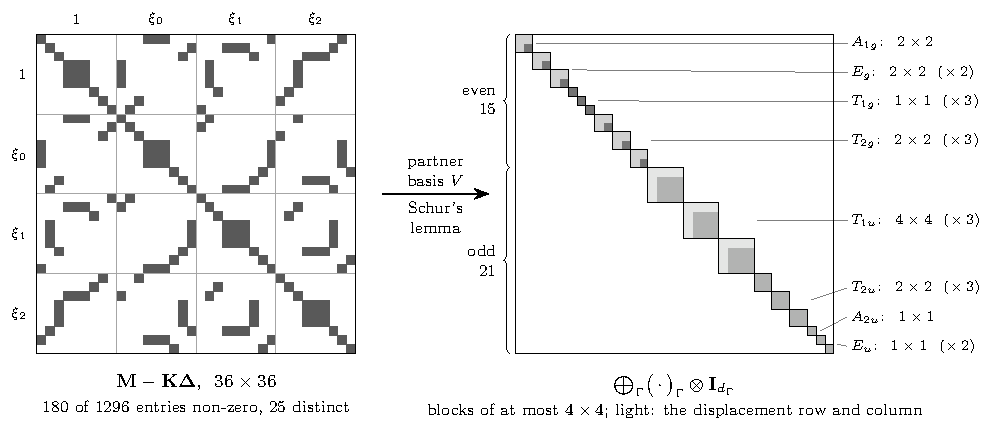
\includegraphics[width=\linewidth]{figures/fig_blocks.pdf}
\caption{The single-site system before and after the change to the partner basis. Left: the non-zero
entries of $\bM-\bK\bD$ (dark) in the natural ordering, the four functions $1,\xi_0,\xi_1,\xi_2$ each
carrying the nine components, at $k_Sh=0.1$; $180$ of the $1296$ entries are non-zero, and they take only
$25$ distinct values up to sign, the symmetry of the cube repeating them within and between the blocks of
the functions. Right: the same matrix in the basis of partner vectors (Table~\ref{tab:vectors}),
by Schur's lemma block diagonal, Eq.~\eqref{eq:t36blocks}: each irreducible representation gives one block,
of size its multiplicity, repeated once for each of its rows; the $15$ even unknowns (darker) never couple
to the $21$ odd (lighter). The same structure holds at every frequency and for every power of $k_Sh$, and
for $\bT_{36}$.}
\label{fig:blocks}
\end{figure} Appendix~\ref{app:group} gives the group's action on the unknowns,
why the commutation holds, Schur's lemma and what it requires, and the vectors that span one row of each
block (Table~\ref{tab:vectors}); the reduction is exact, with no residual at any power computed
(\S\ref{sec:checks}).

On each representation
\begin{equation}\label{eq:tgamma}
  \bT_\Gamma=M_\Gamma\bD_\Gamma\bigl(\bI-\bN_\Gamma\bD_\Gamma\bigr)^{-1},\qquad
  \bN_\Gamma=\frac1\mu\sum_{n\ge0}(k_Sh)^n\,\mathrm i^n\Bigl[\frac{\mathbf P_{\Gamma,n}}{n!}
  -\bigl(1-\gamma^{n+2}\bigr)\frac{\mathbf Q_{\Gamma,n}}{(n+2)!}\Bigr],
\end{equation}
with $\bD_\Gamma$ the contrast on the vectors of $\Gamma$, which is $\omega^2\Delta\rho$ on a displacement
vector and a combination of $\Delta\lambda$ and $\Delta\mu$ on a strain vector, and $\mathbf P_{\Gamma,n}$,
$\mathbf Q_{\Gamma,n}$ the reduced forms of $\mathbf A_n$ and $\mathbf B_n$ divided by $4\pi M_\Gamma$. Each
of their entries is a rational vector on the six constants (\S\ref{sec:constants}); all of them, through
the highest power computed, are in \path{data/self_blocks_irreps.txt}. As an example, the uniform
dilatation ($A_{1g}$, the strain vector) has $P_{0}=-\tfrac13$ and $Q_{0}=-\tfrac23$, so that its static
entry is $\mu N=-\tfrac13+\tfrac12(1-\gamma^2)\tfrac23=-\gamma^2/3$, that is
$N=-1/[3(\lambda+2\mu)]$, the value for every shape \citep{NestorCoupling2026}; all $36$ static entries
of the uniform and linear strain reproduce those of \citet{NestorCoupling2026}, coefficient by coefficient
on its five constants. Its first
dynamic correction is
\begin{equation}\label{eq:a1gdyn}
  \mu N_{A_{1g},2}[\varepsilon,\varepsilon]=-\frac{1}{2}\Bigl[P_2-\frac{1-\gamma^4}{12}Q_2\Bigr],\qquad
  \pi P_2=\tfrac4{15}-\tfrac49\pi+\tfrac4{15}\sqrt2-\tfrac8{15}\sqrt3+\tfrac43\ln(1+\sqrt2)
  +\tfrac43\ln(2+\sqrt3),
\end{equation}
and likewise for $Q_2$ (the data file); $(k_Sh)^2$ times this is the leading change with frequency of
the cell's dilatational self-interaction.

\section{Checks}\label{sec:checks}

Every step is checked against an evaluation that shares none of it
(\path{scripts/derive_legendre_cell_dynamic.py}), with the background $\alpha=5000$\,m\,s$^{-1}$,
$\beta=3000$\,m\,s$^{-1}$, $\rho=2500$\,kg\,m$^{-3}$ and the contrast $\Delta\lambda=2$\,GPa,
$\Delta\mu=1$\,GPa, $\Delta\rho=100$\,kg\,m$^{-3}$. Table~\ref{tab:checks} gives the results.

\begin{table}[htbp]
\centering
\caption{Checks of the closed form through $(k_Sh)^6$. The reference for the series is the package's
series of the self block (master integrals at forty digits for odd $m$, Gauss rules for even $m$), which
itself agrees with quadrature of the singular integrals to $1.4\times10^{-15}$.}\label{tab:checks}
\small
\begin{tabular}{@{}p{8.6cm}l@{}}
\toprule
check & result \\
\midrule
$223$ exact moments, $m=-1$ to $7$, against the package's & $1.7\times10^{-15}$ \\
self block, exact series to $n=6$, against the full series, $k_Sh=0.02,0.05,0.1,0.2$ &
$1.1\times10^{-14}$, $6.6\times10^{-12}$, $8.4\times10^{-10}$, $1.1\times10^{-7}$ \\
\quad apparent order of that difference & $7.00$ \\
$\bT_{36}$ from the exact series against $\bT_{36}$ by quadrature, $k_Sh=0.05,0.1,0.2$ &
$2.1\times10^{-13}$, $2.7\times10^{-11}$, $3.5\times10^{-9}$ \\
\quad apparent order & $7.00$ \\
\quad the same truncated at $n=4$ & $5.9\times10^{-10}$, $1.9\times10^{-8}$, $6.1\times10^{-7}$; order $5.00$ \\
invariance of every representation's span under every $\bK_n$ & exact (no residual) \\
$\bT_{36}V_\Gamma=V_\Gamma\bT_\Gamma$, Eq.~\eqref{eq:tgamma}, worst over $\Gamma$, $k_Sh=0.05,0.1,0.2$ &
$4.4\times10^{-13}$, $5.6\times10^{-11}$, $7.2\times10^{-9}$ \\
static uniform dilatation & $-1/[3(\lambda+2\mu)]$ exactly \\
the $36$ static strain entries against \citet{NestorCoupling2026} & identical coefficients \\
radiation at $n=1$ & $\mathrm{Im}\,\bG(0)$ exactly, Eq.~\eqref{eq:radiation} \\
\bottomrule
\end{tabular}
\end{table}

The differences fall as $(k_Sh)^7$, the first power omitted (and as $(k_Sh)^5$ when the series stops at
$n=4$), so they are the truncation of the series and
not an error of its terms. The closed form is that of the exact self block: what it omits at a given order
is stated by the next term, which is itself in closed form.

\section{Discussion}\label{sec:discussion}

\paragraph{A frequency sweep with no integral at any frequency.} The single-site $T$-matrix of the linear
Legendre cell is now known in closed form at every power of the frequency, and what that buys is a sweep. The
coefficients $\bK_n$ depend on neither the frequency, the cell size nor the medium: they are computed once,
in exact arithmetic, and stored. At each frequency the self block is then the polynomial
$\sum_n(k_Sh)^n\bK_n$, scaled to the cell by Eq.~\eqref{eq:kseries}, and the $T$-matrix one $36\times36$
solve, or eight solves of at most $4\times4$ on the irreducible representations. Nothing singular is
integrated at any frequency. Measured on one machine (\path{scripts/measure_legendre_cell_sweep.py}),
one frequency costs $0.29$\,ms by the closed form against $2.0$\,s by quadrature of the singular self
integrals, a factor of about $7000$, and against $16$\,ms by the package's numerical series of the same
moments. The one-off cost of the closed form, the $223$ exact moments and their assembly and reduction
through $(k_Sh)^6$, is $30$\,s on four cores, paid once for every cell, frequency and medium; against
quadrature it is recovered after about fifteen frequencies, and a sweep of a thousand frequencies that
quadrature would take half an hour to tabulate costs half a minute in all. The coupling between cells has
the same structure \citep{NestorCoupling2026}: its coefficients too are universal and computed once, and over
$1024$ frequencies its series costs $6$ to $13$\,min against $34$ to $89$\,min by quadrature on the grids
measured there. With both, a model of cells is assembled at any frequency from stored numbers.

\paragraph{The range of the truncated series.} The series converges for every $k_Sh$, but a sweep
evaluates it truncated. The figures that follow are for the single-site $T$-matrix of one cell, compared entry
by entry (largest difference relative to the largest entry) with the same $T$-matrix built on the self block
by quadrature. The cell's interaction with its own field is summed exactly by the inverse in
Eq.~\eqref{eq:t36}, and no other cell is involved: the truncation is only that of the series in the frequency
of the self block. Through $(k_Sh)^6$ the $T$-matrix is accurate to $3.5\times10^{-9}$ at $k_Sh=0.2$,
$5.9\times10^{-8}$ at $0.3$, $2.1\times10^{-6}$ at $0.5$ and $2.6\times10^{-4}$ at $1$, against quadrature
that agrees with the package's series to $10^{-16}$; stopping at $(k_Sh)^4$ instead loses three orders of
magnitude at $k_Sh=0.05$ and less than one at $k_Sh=1$. A discretisation with ten cells to the shear
wavelength has $k_Sh=\pi/10\approx0.31$, where the truncation through $(k_Sh)^6$ leaves $8.2\times10^{-8}$. Beyond that, the next powers are in closed form like the
first, from the same derivation, at a one-off cost that grows with the number of moments.

\paragraph{What is not yet covered.} Two things. The contrast here is uniform in the cell; a graded contrast couples the
even and odd unknowns and leaves only the operations that fix its gradient
\citep{NestorCoupling2026}, so the reduction is weaker, though the moments are the same and the closed
form carries over. And the field is linear; the quadratic cell of $90$ unknowns needs the moments of
monomials to degree four, which the same derivation provides. The comparison with the single site of the
expansion about the centre, whose self-interaction is taken at the centre rather than averaged over the
cell \citep{NestorContinuum2026,NestorCoupling2026}, is to be condensed here from the earlier paper.

\section*{Data availability}
The derivation and its checks are \path{scripts/derive_legendre_cell_dynamic.py}, which writes
\path{data/self_moments_exact.pkl} (every moment, exact) and \path{data/self_blocks_irreps.txt} (every
reduced entry, on the six constants), in the repository
\url{https://github.com/tmnestor/MultipleScatteringCalculations}. The cost of a sweep and the range of the
truncated series are measured by \path{scripts/measure_legendre_cell_sweep.py}. The static blocks are
\path{scripts/derive_graded_voxel_site_blocks.py}.

\appendix

\section{The cube group and Schur's lemma}\label{app:group}

The splitting of \S\ref{sec:group} rests on Schur's lemma from the representation theory of finite groups
\citep{Tinkham1964,Dresselhaus2008}. This appendix sets out the group's action on the unknowns of the cell,
why the cell's matrices commute with it, and the form the lemma then gives them.

\paragraph{Symmetries of the cube.} A \emph{symmetry} of the cube is a linear map $\bxi\mapsto Q\bxi$ of
space that preserves distances and maps the cube $[-1,1]^3$ onto itself; it fixes the centre, and $Q$ is an
orthogonal matrix, $Q^{\mathsf T}Q=\bI$. Such a map must send the six face centres $\pm\mathbf e_j$ to face
centres, so each column of $Q$ is some $\pm\mathbf e_i$: $Q$ is a \emph{signed permutation matrix}, a
permutation of the three axes combined with a choice of sign for each. There are $3!\times2^3=48$ of them,
the rotations of the cube ($\det Q=+1$) and their products with the inversion $\bxi\mapsto-\bxi$
($\det Q=-1$), which include the reflections in the coordinate and diagonal planes. The product of two
symmetries and the inverse $Q^{-1}=Q^{\mathsf T}$ of one are again symmetries, so they form a group, the
octahedral group $O_h$. For example, the quarter turn about axis $0$ and the reflection in the plane
$\xi_0=0$ are
\begin{equation}\label{eq:qexample}
  Q_{\mathrm{turn}}=\begin{pmatrix}1&0&0\\0&0&-1\\0&1&0\end{pmatrix},\qquad
  Q_{\mathrm{refl}}=\begin{pmatrix}-1&0&0\\0&1&0\\0&0&1\end{pmatrix}.
\end{equation}

\paragraph{How a symmetry acts on the field of the cell.} Applying $Q$ to a field carries the value at
$\bxi$ to $Q\bxi$ and turns its components with it: the displacement is a vector, $u\mapsto Qu$, and the
strain a symmetric tensor, $\varepsilon\mapsto Q\varepsilon Q^{\mathsf T}$, that is
$\varepsilon'_{ij}=\sum_{k,l}Q_{ik}Q_{jl}\varepsilon_{kl}$. On the nine components $\psi=(u,\varepsilon)$
this is the $9\times9$ matrix
\begin{equation}\label{eq:sq}
  S(Q)=\begin{pmatrix}Q&0\\0&\Sigma(Q)\end{pmatrix},
\end{equation}
with $\Sigma(Q)$ the $6\times6$ matrix of $\varepsilon\mapsto Q\varepsilon Q^{\mathsf T}$ in Voigt form. The
transformed field is $\psi'(\bxi)=S(Q)\,\psi(Q^{\mathsf T}\bxi)$. For the cell's field
$\psi(\bxi)=\sum_b\psi_bL_b(\bxi)$ the functions are moved as well: $1$ is unchanged, and
$L_{k}(Q^{\mathsf T}\bxi)=(Q^{\mathsf T}\bxi)_k=\sum_jQ_{jk}\,\xi_j$ for the linear functions
$L_k=\xi_k$. So the four functions are mixed by the $4\times4$ matrix
\begin{equation}\label{eq:tq}
  T(Q)=\begin{pmatrix}1&0\\0&Q\end{pmatrix},
\end{equation}
and the coefficients of the transformed field are
\begin{equation}\label{eq:coefmap}
  \psi'_a=\sum_{b=0}^{3}T_{ab}(Q)\,S(Q)\,\psi_b ,\qquad a=0,\dots,3.
\end{equation}
Two things happen at once and independently: $T(Q)$ mixes \emph{which function} carries the field, and
$S(Q)$ mixes \emph{which component} of the field it is.

\paragraph{The Kronecker product.} Stack the $36$ unknowns as one column,
$\Psi=(\psi_0,\psi_1,\psi_2,\psi_3)$, each $\psi_b$ nine components, so that the unknown with function
index $a$ and component $i$ sits in row $9a+i$. Eq.~\eqref{eq:coefmap} is then $\Psi'=D(Q)\Psi$ with the
$36\times36$ matrix
\begin{equation}\label{eq:rep}
  D(Q)=T(Q)\otimes S(Q)=\begin{pmatrix}
    T_{00}S&T_{01}S&T_{02}S&T_{03}S\\
    T_{10}S&T_{11}S&T_{12}S&T_{13}S\\
    T_{20}S&T_{21}S&T_{22}S&T_{23}S\\
    T_{30}S&T_{31}S&T_{32}S&T_{33}S
  \end{pmatrix},\qquad
  D(Q)_{9a+i,\,9b+j}=T_{ab}(Q)\,S_{ij}(Q),
\end{equation}
the Kronecker product: the $4\times4$ array of $9\times9$ blocks whose block $(a,b)$ is $S(Q)$ scaled by
the number $T_{ab}(Q)$. It is the matrix of a map that acts on the function index by $T$ and on the
component index by $S$, each without regard to the other. For the reflection of Eq.~\eqref{eq:qexample},
$T=\operatorname{diag}(1,-1,1,1)$, and $S$ is diagonal with $-1$ on $u_0$ and on the shears
$\varepsilon_{01}$ and $\varepsilon_{02}$, which change sign with $\xi_0$, and $+1$ elsewhere; so $D$ is
diagonal, and the sign of the unknown $\xi_0u_0$, for instance, is $T_{11}S_{00}=(-1)(-1)=+1$. Because the
Kronecker product satisfies $(A\otimes B)(C\otimes F)=AC\otimes BF$, and $T$ and $S$ each respect products,
\begin{equation}\label{eq:homomorphism}
  D(Q_1)\,D(Q_2)=D(Q_1Q_2)\qquad\text{for all }Q_1,Q_2\in O_h:
\end{equation}
the assignment $Q\mapsto D(Q)$ turns composition of symmetries into multiplication of matrices, which is
what is meant by a \emph{representation} of the group. For a signed permutation, $Q\varepsilon Q^{\mathsf T}$
permutes the strain components with signs and sends shears to shears, so $\Sigma(Q)$, $S(Q)$, $T(Q)$ and
$D(Q)$ are all signed permutation matrices, and orthogonal: $D(Q)^{-1}=D(Q)^{\mathsf T}=D(Q^{\mathsf T})$.

\paragraph{Why the cell's matrices commute with it.} Three facts make
\begin{equation}\label{eq:commute}
  D(Q)\,\bK\,D(Q)^{\mathsf T}=\bK,\qquad D(Q)\,\bM\,D(Q)^{\mathsf T}=\bM,\qquad D(Q)\,\bD\,D(Q)^{\mathsf T}=\bD
  \qquad\text{for all $48$ }Q.
\end{equation}
\emph{The domain is invariant}: $Q$ maps the cube onto itself. \emph{The kernel is covariant}: the
background is isotropic, so its Green's tensor satisfies $\bG(Q\mathbf r)=Q\,\bG(\mathbf r)\,Q^{\mathsf T}$
for every orthogonal $Q$, reflections included, and its derivatives transform as tensors of the
corresponding rank; changing variables $\bx\mapsto Q\bx$, $\by\mapsto Q\by$ in the double integral of
$\bK$ then gives the first identity. \emph{The contrast is invariant}: uniform in the cell, $\omega^2\Delta\rho$ is a
scalar and $\delta c$ an isotropic tensor, so $\bD$ commutes with $S(Q)$; and the Gram matrix $\bM$ only
weights the functions $1$ and $\xi_i$, which $Q$ permutes among themselves with equal weights. The system
matrix $\bM-\bK\bD$, its inverse, and $\bT_{36}$ of Eq.~\eqref{eq:t36} therefore commute with every
$D(Q)$. Nothing here requires $\bK$ to be Hermitian or real: the identities hold for the complex self block
at every frequency, radiation included, and power by power for each $\bK_n$.

\paragraph{Schur's lemma.} A representation is \emph{irreducible} when no subspace other than $0$ and the
whole is mapped into itself by every $D(Q)$. Schur's lemma states that a linear map between two irreducible
representations that commutes with the group action is zero if the representations are inequivalent, and a
multiple of the identity if they are the same. The $36$-dimensional representation of Eq.~\eqref{eq:rep} is
not irreducible; it is a direct sum of copies of the ten irreducible representations of $O_h$, labelled by
their dimension ($A$: $1$, $E$: $2$, $T$: $3$) and by their parity under the inversion $\bxi\mapsto-\bxi$
($g$ even, $u$ odd). How many copies $n_\Gamma$ of each $\Gamma$ occur follows from the characters, the
traces of the representation matrices: $n_\Gamma=\tfrac1{48}\sum_Q\chi_\Gamma(Q)\operatorname{tr}D(Q)$, with
$\operatorname{tr}D(Q)=\operatorname{tr}T(Q)\operatorname{tr}S(Q)$. Every irreducible representation of $O_h$
can be written with real matrices and has real characters, so the lemma holds over the real numbers, and
applies to the real and imaginary parts of $\bK$ alike. Applied to an operator that commutes with $D(Q)$, it
has two consequences. First, the operator does not couple unknowns of different $\Gamma$. Second, within the
$n_\Gamma$ copies of a $\Gamma$ of dimension $d_\Gamma$, if a basis is chosen in which every copy is
represented by the \emph{same} matrices (each basis vector a \emph{partner}, transforming as a given row of
$\Gamma$), the operator acts as an $n_\Gamma\times n_\Gamma$ matrix on the multiplicity index and as the
identity on the row index, which is Eq.~\eqref{eq:schur}, and likewise for $\bM$, $\bD$, $\bM-\bK\bD$ and $\bT_{36}$. The block $\bK_\Gamma$ is then found from any one
row: with $V_\Gamma$ the $36\times n_\Gamma$ matrix whose columns are the partners of that row,
$\bK V_\Gamma=V_\Gamma\bK_\Gamma$. Inverting the $36\times36$ system reduces to inverting $n_\Gamma\times
n_\Gamma$ blocks, of size at most $4\times4$.

\paragraph{The partners.} Table~\ref{tab:vectors} gives the partners of one
row of each $\Gamma$ as integer vectors. They are chosen so that within each $\Gamma$ they transform alike:
the displacement's first moment $\xi_1u_2+\xi_2u_1$ and the shear $2\varepsilon_{12}$, for instance, both
transform as the $(1,2)$ row of $T_{2g}$. The reduction is then exact: $\bK_nV_\Gamma=V_\Gamma\bK_{\Gamma,n}$
with no residual at any power computed (\S\ref{sec:checks}).

\begin{table}[htbp]
\centering
\caption{One row of each irreducible representation, as combinations of the unknowns $\xi_iu_j$ ($L_b=\xi_i$
times the displacement component $j$), $u_j$, $\varepsilon_{ij}$ and $\xi_i\varepsilon_{jk}$, axes
$0,1,2$.}\label{tab:vectors}
\small
\begin{tabular}{@{}lll@{}}
\toprule
$\Gamma$ & vectors & $M_\Gamma/h^3$ \\
\midrule
$A_{1g}$ & $\xi_0u_0+\xi_1u_1+\xi_2u_2$; \ $\varepsilon_{00}+\varepsilon_{11}+\varepsilon_{22}$ & $\tfrac83,8$\\
$E_g$ & $2\xi_0u_0-\xi_1u_1-\xi_2u_2$; \ $2\varepsilon_{00}-\varepsilon_{11}-\varepsilon_{22}$ & $\tfrac83,8$\\
$T_{1g}$ & $\xi_1u_2-\xi_2u_1$ & $\tfrac83$\\
$T_{2g}$ & $\xi_1u_2+\xi_2u_1$; \ $2\varepsilon_{12}$ & $\tfrac83,8$\\
$T_{1u}$ & $u_0$; \ $\xi_0\varepsilon_{00}$; \ $\xi_0(\varepsilon_{11}+\varepsilon_{22})$; \
$2(\xi_1\varepsilon_{01}+\xi_2\varepsilon_{02})$ & $8,\tfrac83,\tfrac83,\tfrac83$\\
$T_{2u}$ & $\xi_0(\varepsilon_{11}-\varepsilon_{22})$; \ $2(\xi_1\varepsilon_{01}-\xi_2\varepsilon_{02})$ & $\tfrac83,\tfrac83$\\
$A_{2u}$ & $2(\xi_0\varepsilon_{12}+\xi_1\varepsilon_{02}+\xi_2\varepsilon_{01})$ & $\tfrac83$\\
$E_u$ & $2(\xi_1\varepsilon_{02}-\xi_2\varepsilon_{01})$ & $\tfrac83$\\
\bottomrule
\end{tabular}
\end{table}


\bibliographystyle{unsrtnat}
\bibliography{references}

\end{document}
